\part{Contexte métier}

    \chapter{Description du Groupe}

    \large
    L'objet de l'ensemble de cette première partie est de donner sur le Groupe Pomona des éclairages nécessaires à la compréhension du cas d'usage développé.
    Bien d'autres aspects sur la société, pourraient être mentionnés (ex : des indicateurs sur l'activité, l'histoire du Groupe\dots) mais ils seront omis car non indispensables à la compréhension du sujet.
    Plus de détails sur le Groupe sont accessibles sur le site web de la société\cite{site_pomona}.
    \normalsize    

        \section{Le métier du Groupe Pomona}

        Le Groupe Pomona est une société de distribution livrée de produits alimentaires à destination des professionnels des métiers de bouche.
        L'activité du Groupe consiste uniquement à acheter et revendre de la marchandise, à l'exclusion de toute activité de fabrication ou de transformation\footnote{de très rares cas de transformation existent (ex : mûrissage de fruits, filetage de poisson) mais sont extrêmement exceptionnels}. Le Groupe Pomona est une société de \emph{distribution}. Elle ne possède d'ailleurs pas d'actif industriels (autre que des entrepôts logistiques) ni d'agréement pour transformer les marchandises.        
        
        Cette activité d'achat/vente se fait dans la majorité des cas sous le régime du \emph{négoce}, à savoir que le Groupe acquiert la propriété des marchandises qu'il commercialise avant de la céder à ses clients.
        L'autre régime est celui dit de la \emph{prestation (logistique)}.
        Dans ce cas, par le jeux d'écritures comptables, la valorisation du stock disparaît des comptes du Groupe.
        Néanmoins, indépendamment de cet aspect purement comptable, l'ensemble :
        \begin{description}
            \item[des flux de documents :] commandes d'achat, factures fournisseur, commandes de vente, factures clients
            \item[des flux financiers :] paiements fournisseur, paiements client
            \item[des flux physiques :] réception et stockage, préparation et expédition
        \end{description}
        restent largement inchangés.
        
        Pour résumer, l'activité de l'ensemble des entités du Groupe pourraient se résumer via le schéma présenté en figure \ref{fig:flux metier}

        \begin{figure}[htbp]
            \begin{center}
            \includegraphics[width=\linewidth]{img/Les flux métier de Pomona.png}
            \end{center}
            \caption{Les flux métier avec les partenaires commerciaux}
            \label{fig:flux metier}
        \end{figure}

        \emphbox{Le métier du Groupe est d'être un \emph{grossiste}, qui achète et revend des produits alimentaires\footnotemark \ \emph{sans produire ou transformer quoi que ce soit}.}
        \footnotetext{dans la grande majorité des cas, cf. paragraphe \emph{Les produits non-alimentaires} page \pageref{produits_nonal}}

        \section{La décentralisation}
        
        Le Groupe Pomona est un Groupe fortement décentralisé, avec des organisations largement indépendantes les unes des autres. 

            \subsection{Les Directions fonctionnelles}

            Pour des raisons évidentes de recherche de synergies ou de conformité réglementaires, certaines activités restent toutefois mutualisées à la maille du Groupe.
            Il s'agit des organisations suivantes :
            \begin{description}
                \item[La Direction Administrative et Financière (DAF) :] regroupe les équipes comptables Groupe, l'audit interne et la consolidation financière
                \item[La Direction Qualité :] est en charge de définir et contrôler l'application des standard de qualité
                \item[La Direction des Systèmes d'Information (DSI) :] développe et maintient en condition opérationnelles les systèmes d'information du Groupe
                \item[La Direction Technique et Logistique (DTL) :] est en charge des projets immobiliers (entrepôts), des négociations avec les transporteurs et joue un rôle de conseil interne sur les sujets logistiques
                \item[La Direction des Ressources Humaines :] se charge de l'ensemble des aspects en lien avec le recrutement, la paye et les sujets sociaux
                \item[La Direction Commerciale Groupe (DCG) :] définit une stratégie et des bonnes pratiques commerciales et marketing
            \end{description}

            \subsection{Les clients du Groupe}
            \label{clients}

            Afin de comprendre l'organisation du Groupe, il est nécessaire de connaître la typologie de ses clients.
            Comme mentionné précédemment, le Groupe s'adresse exclusivement aux professionnels des métiers de bouche.
            Aucune marchandise n'est vendue à des particuliers.
            Les principales typologies de clients sont les suivantes : 
            \begin{description}
                \item[Les Sociétés de Restauration :] elles exploitent les restaurants d'entreprise et certaines cantines d'établissement d'enseignement supérieur
                \item[Les Marchés Publics :] regroupent les clients qui dépendent des collectivités (écoles, hôpitaux, prisons, \dots)
                \item[La restauration commerciale :] est l'ensemble des restaurants à vocation commerciale, qu'ils soient chaînés (hippopotamus, O'Tacos, \dots) ou indépendants (\og le restaurant du coin \fg)
                \item[Les spécialistes :] il s'agit des détaillants spécialisés qui s'adressent aux particuliers. Boulangers, pâtissiers, bouchers, traiteurs, vente à emporter, \dots
                \item[Les Grandes et Moyennes surfaces (la GMS) :] sont les enseignes de la grande distribution. En général, l'accès à ces clients est compliqué par les règles mises en place par leurs centrales d'achat. Il représentent en général qu'un canal de vente d'opportunité.
            \end{description}

            Les trois premières de ces catégories représentent ce que l'on appelle la \emph{Restauration Hors Domicile (RHD)} (ou parfois également la Restauration Hors Foyer, RHF).

            \subsection{Premier niveau de décentralisation : les branches}
            
            Le Groupe Pomona est divisé en branches, qui sont des organisations indépendantes et qui ont toute latitude pour gérer leurs stratégie et politique commerciales, la gestion de leurs achats, leur stratégie marketing, \dots
            Afin d'éviter de se concurrencer entre elles, leurs domaines d'activité respectifs ont été partitionnés par familles de produit commercialisés, segments client cibles et géographie. 

                \subsubsection{Les branches RHD}
                
                Les branches RHD s'adressent comme leur nom l'indique aux client de la Restauration Hors Domicile (cf. section \ref{clients} page \pageref{clients}) en France.
                Elles se répartissent ce marché en travaillant des gammes de produits distinctes.
                Il s'agit des branches historiques du Groupe, qui représentent l'essentiel de son chiffre d'affaire.
                La répartition par produit est la suivante :
                \begin{description}
                    \item[PassionFroid :] spécialiste des \emph{produits surgelés, de la viande fraîche et des produits laitiers}
                    \item[\'{E}piSaveurs :] spécialiste des produits qui se conservent à température ambiante : \emph{produits d'épicerie, conserves, boissons et consommables de cuisine non-alimentaires}
                    \item[TerreAzur :] spécialites des \emph{Fruits et Légumes frais, et Produits De la Mer frais} 
                \end{description}
                La non-concurrence entre les branches est assurée par le fait qu'elles ne commercialisent pas les mêmes produits.
                Bien que nommées RHD, elles peuvent également vendre leurs produits à la grande distribution, mais généralement ces marchés sont verrouillés par les centrales d'achat des grandes enseignes.

                \subsubsection{Les branches spécialistes}

                Les branches spécialistes s'adressent aux clients dits spécialistes (cf. section \ref{clients} page \pageref{clients}) en France.
                Elles sont en mesure de commercialiser tout type de produit pour répondre aux besoins de leurs clients.
                En particulier, elles peuvent tout à fait commercialiser certains produits qui sont également vendus par les branches RHD.
                Elles se répartissent la clientèle spécialiste de la manière suivante :
                \begin{description}
                    \item[Délice et Création :] s'addresse aux \emph{Boulangers et Pâtissiers}
                    \item[Saveurs d'Antoine :] s'adresse aux \emph{Bouchers, Charcutiers et Traiteurs}
                    \item[Relais d'Or :] s'addresse à la \emph{restauration indépendante nomade}
                \end{description}
                Comme pour les branches RHD, ces branches peuvent lorsqu'elles en ont l'opportunité vendre leurs produits à la GMS.

                \subsubsection{L'étranger}

                Bien que le Groupe Pomona soit une société dont l'essentiel de l'activité est faite sur le marché français, deux réseaux sont en cours de constitution sur des pays limitrophe.
                Ces branches sont susceptibles de travailler tout type de produit, à destination de tout type de client.
                Elles sont positionnées sur les marchés suivants : 
                \begin{description}
                    \item[Pomona Suisse :] présente sur le marché Suisse
                    \item[Pomona Iberia :] présente sur le marché Espagnol 
                \end{description}

                On peut synthétiser la répartition de l'activité par branche de la manière présentée à la figure \ref{fig:repartition_activite}.

                \subsubsection{Les produits non-alimentaires}
                \label{produits_nonal}
                Si l'essentiel des produits commercialisés par les branches du Groupe sont des produits alimentaires, comme évoqué précédemment une partie de l'activité commerciale se fait tout de même autour de produits non-alimentaires.
                Ces produits restent malgré tout destinés exclusivement aux professionnels des métier de bouche, et il s'agit de consommables (par opposition à des articles d'électroménager, de la vaisselle non-jetable, \dots).

                On distingue en général deux catégories de produits non-alimentaires : 
                \begin{itemize}
                    \item les produits dits \og d'hygiène \fg
                    \item les produits dits \og de chimie \fg
                \end{itemize}

                Les produits de chimie regroupent les produits qui doivent faire l'objet d'une fiche de données de sécurté au sens du réglement Européen No 1907/2006 dit \og REACH \fg (Registration, Evaluation, Authorisation and Restriction of Chemicals) \cite{reach_text}.

                Les produits d'hygiène regroupent tous les autres produits non-alimentaires.
                L'appelation \og d'hygiène \fg est donc réductricte, dans la mesure où cette large famille regroupe les consommables de nettoyage (éponges, papiers absorbants, \dots) mais également tout type d'autres consommables (serviettes de tables, gobelets en plastiques, pics à brochettes, boîtes de produits à emporter, \dots).

                \emphbox{La commercialisation de produits non-alimentaires existe au sein du Groupe, mais on se focalisera pour la suite sur les produits alimentaires qui reste le coeur de métier.}

                \begin{figure}[htpb]
                    \begin{center}
                    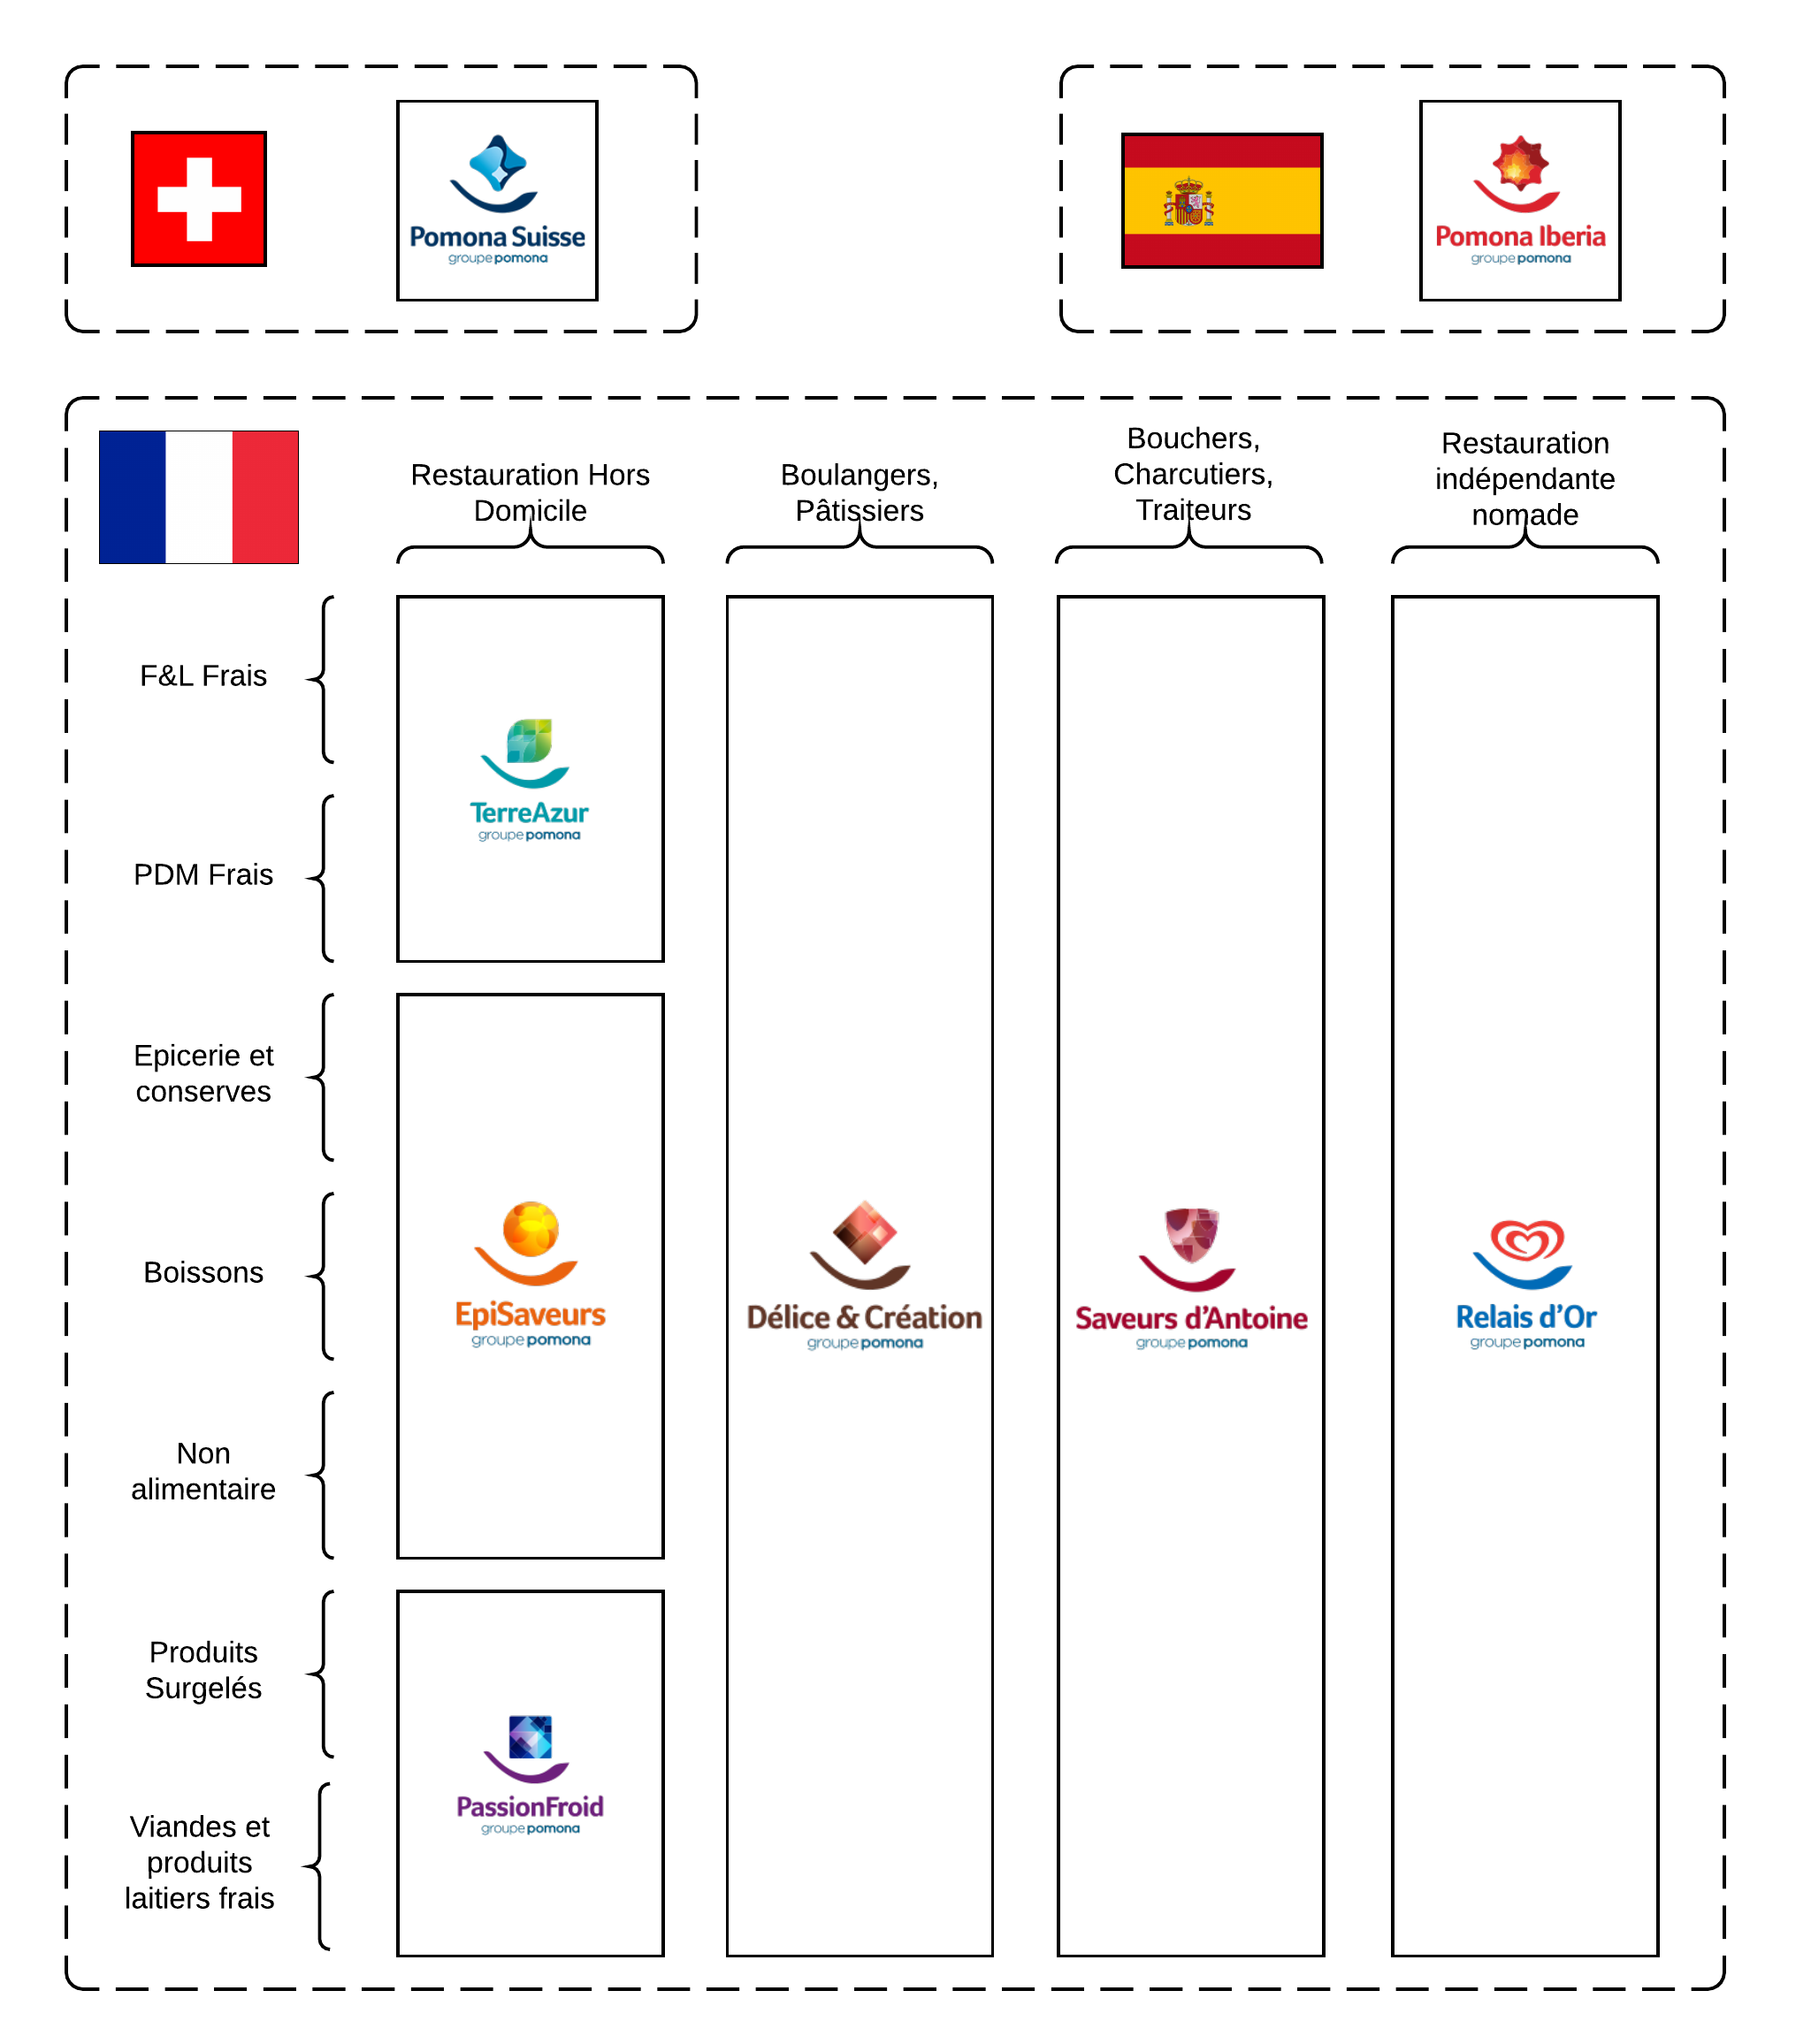
\includegraphics[width=\linewidth]{img/La répartition de l'activité des branches.png}
                    \end{center}
                    \caption{La répartition de l'activité des branches}
                    \label{fig:repartition_activite}
                \end{figure}

            \subsection{Le second niveau de décentralisation : les succursales}

            Chacune des branches est elle-même à son tour décentralisée en un réseau d'entrepôts régionaux : les succursales (parfois également appelées simplement \og régions\fg).
            Ces succursales sont gérées comme des PME indépendantes, avec un directeur et un compte de résultat qui leur est propre.
            Si certaines négociation avec des fournisseurs ou des clients nationaux sont parfois menée par les branches, les succursales sont autonomes dans :
            \begin{itemize}
                \item{la définition de leur assortiment, même si des contraintes s'appliquent}
                \item{la stratégie de développement commercial}
                \item{la négociation des prix d'achat}
                \item{la négociation des prix de vente}
                \item{la politique de rémunération de leurs employés}
            \end{itemize}
            
            \'{A} ce titre, elles ont leurs propres équipes d'achat, leurs équipes commerciales (télévente et vente route), leurs équipes administratives et évidemment leurs équipes logistiques (essentiellement en entrepôt et les chauffeurs livreurs en charge des livraisons client).
            Un exemple de maillage régional est présenté en figure \ref{fig:reseau_es}, sachant que ce maillage régional est différent pour chacune des branches.
            \begin{figure}[htpb]
                \begin{center}
                \includegraphics[width=\linewidth]{img/réseau es.png}
                \end{center}
                \caption{Le maillage régional de la branche \'{E}piSaveurs}
                \label{fig:reseau_es}
            \end{figure}


    \chapter{La gestion de l'information produit}
    
    \large
    Ce chapitre a pour vocation à éclairer les aspects métier en lien avec la gestion de l'information produit. 
    C'est le seul processus métier qui sera détaillé dans la mesure où c'est uniquement celui qu'il est nécessaire de connaître pour comprendre les cas d'usage développés ultérieurement.
    \normalsize

        \section{L'information produit}
        
            \subsection{Utilisations de l'information produit}
        
                \subsubsection{Conformité réglementaire}
                La gestion de l'information produit est essentiellement une contrainte réglementaire à statisfaire.
                Comme mentionné au préambule, la réglementation autour de l'information des consommateur s'est sans cesse complétée au cours des dernières années.
                Un des textes centraux est le règlement n°1169/2011 dit INCO (INformation COnsommateur)\cite{incotext}\cite{incoexpl}.
                C'est ce règlement qui définit l'ensemble des informations qui doivent être étiquetées sur le produit (liste d'ingrédients, tableau de données nutritionnelles, \dots), mais également affichée au client lors de commande en ligne sur les sites de e-commerce.
                Il s'agit principalement d'informations relatives à la sécurité alimentaire (ex : les allergènes) ou la santé (ex : informations nutritionnelles).

                \subsubsection{Attentes client}

                Les consommateurs finaux (les \og convives \fg) étant de plus en plus sensibles au contenu de leur assiète, les clients du Groupe sont de plus en plus demandeurs d'information relatives aux produits qu'ils commandent.
                Ils demandent donc régulièrement des informations qui vont au-delà de ce qui est normalement prévu par la réglementaition.

                De plus, sur certains marchés pour lesquels des contrats courant sur de longues périodes - jusqu'à un an - sont établis (les marchés publics sont très concernés), il n'y a pas d'échantillonnage des produits.
                La seule manière pour ces clients d'évaluer la qualité des produits est de se référer aux documents contenant les informations produit, fournis par les distributeurs.

                \subsubsection{Gestion}

                Certaines informations relatives au produits sont nécessaires pour des raison de gestion adminsitrative.
                Par exemple, la gestion des taxes sur les produits alimentaires est complexe : 
                \begin{itemize}
                    \item les taux de TVA sont variables en fonction du type de produit
                    \item des taxes spécifiques s'appliquaient aux produits contenant de l'huile ou de la farine
                    \item des règlements particuliers s'appliquent aux alcools
                    \item \dots
                \end{itemize}
                D'autres informations, comme la nomenclature douanière, sont nécessaires pour effectuer les déclarations auprès des douanes européennes.

                Un autre type d'information capital pour la gestion des flux d'achat et de vente sont les informations logistiques, qui définissent par exemple le nombre d'unités consommateur dans le colis, le nombre de colis sur une palette, \dots
                Une gestion rigoureuse de ces information est indispensable pour que les flux d'achat ou de vente soient correctement exécutés (que les quantités commandées soient les bonnes, que les montants facturés soient corrects, \dots).

            \subsection{Des Produits bruts aux produits transformés}

            Le niveau d'exigence en termes d'information produit est variable en fonction du niveau de transformation de ce produit.
            Par exemple, sur des fruits et légumes frais, à peu de choses près seul le pays d'origine doit être affiché au client.
            Sur une barre chocolatée, ou un plat cuisiné, il sera nécessaire d'afficher :
            \begin{itemize}
                 \item une liste d'ingrédients (mettant en évidence les allergènes)
                 \item un tableau de données nutritionnelles (protéines, gludcides, \dots)
                 \item une dénomination réglementaire
            \end{itemize}

            \subsection{Les grands types d'information}

            On se focalisera dans ce paragraphe sur les informations relatives aux \emph{produits alimentaires}.

                \subsubsection{La composition}

                La première grande famille de données réglementaires sont les données de composition.
                Elles détaillent quels sont les ingrédients qui sont mis en oeuvre dans la fabrication des produits.
                \'{E}videmment, la composition a en général plus de sens que pour les produits transformés que pour les produits bruts.
                Elle peut prendre la forme d'un texte listant la liste des ingrédients (l'étiquetage de ce texte est en général obligatoire sur les emballages des produits), ou d'un tableau.
                
                Les ingrédients incluent également les additifs.
                Il s'agit de substances ajoutées à la recette pour répondre à des fonctions particulières (colorant, exhausteur de goût, émulsifiant).
                Elles ne représentent en général un pourcentage en masse négligeable dans la composition totale du produit.

                Le pourcentage en masse est parfois inclus sur certains ingrédients. 
                La règlementation l'oblige dans certains cas, par exemple quand l'ingrédient en question est mentionné dans la dénomination du produit (pour une \emph{tarte aux framboises}, la proportion de framboise doit être mentionnée dans la composition).

                Enfin, un aspect à la fois règlementaire et particulièrement important est la présence d'allergènes dans la composition.
                Le règlement INCO\cite{incotext}\cite{incoexpl} impose de mettre en évidence les allergènes relevant d'une des 14 catégories suivantes :
                \begin{enumerate}
                    \item Céréales contenant du gluten, à savoir blé, seigle, orge, avoine, épeautre, kamut ou leurs souches hybridées, et produits à base de ces céréales
                    \item Crustacés et produits à base de crustacés
                    \item \OE ufs et produits à base d’ \oe ufs
                    \item Poissons et produits à base de poissons
                    \item Soja et produits à base de soja
                    \item Lait et produits à base de lait (y compris le lactose)
                    \item Fruits à coque, à savoir: amandes, noisettes, noix (Juglans regia), noix de cajou, noix de pécan, noix du Brésil, pistaches, noix de Macadamia ou du Queensland, et produits à base de ces fruits
                    \item Céleri et produits à base de céleri
                    \item Moutarde et produits à base de moutarde
                    \item Graines de sésame et produits à base de graines de sésame
                    \item Anhydride sulfureux et sulfites
                    \item Lupin et produits à base de lupin
                    \item Mollusques et produits à base de mollusques
                \end{enumerate}

                \subsubsection{Les informations nutrionnelles}

                Une autre grande famille d'information produit sont les informations nutritionnelles. 
                Elles détaillent la quantité des principaux nutriments contenus dans les produits.
                Certains d'entre eux sont rendus obligatoires par le règlement INCO\cite{incotext}\cite{incoexpl} cf. l'exemple de tableau \ref{tab:donnees_nut}, et d'autres sont optionnels, comme par exemple la quantité de fer, de calcium, \dots

                \begin{table}
                    \begin{center}
                    \begin{tabularx}{\linewidth}{|X|X|X|X|}
                        \hline
                        \textbf{Informations nutritionnelles} & \textbf{Pour 100g} & \textbf{Pour un biscuit} & \textbf{\% des AJR pour un biscuit} \\
                        \hline
                        \'{E}nergie &1674 kJ\newline398 kcal&209 kJ\newline50 kcal& 3 \% \\
                        \hline
                        Protéines & 3.0 g & 1.0 g & 3 \% \\ 
                        \hline
                        Matières grasses & 13.0 g & 1.6 g & 2 \% \\
                        \hline
                        dont acides gras saturés & 5.8 g & 0.7 g & 4 \% \\
                        \hline
                        Glucides & 66 g & 8.2 g & 3 \% \\
                        \hline
                        dont sucres & 48 g & 6.1 g & 7 \% \\
                        \hline
                        Fibres alimentaires & 2.5 g & 0.3 g &\\
                        \hline
                        Protéines & 3.3 g & 0.4 g & 1 \% \\
                        \hline
                        Sel & 0.41 g & 0.05 g & 1 \% \\
                        \hline
                    \end{tabularx}
                    \end{center}
                    \caption{Exemple de tableau de données nutritionnelles}
                    \label{tab:donnees_nut}
                    Du texte
                \end{table}

                \subsubsection{Les origines}

                \subsubsection{Les données logistiques} 

                \subsubsection{Les données administratives et financières}

            Les allégations

        \section{Le processus associé}
        


        \section{Le PIM (Product Information Management)}
